\documentclass[11pt]{article}

\usepackage[T1]{fontenc}
\usepackage[margin=1in]{geometry} 
\usepackage{amsmath,amsthm,amssymb,amsfonts}

\usepackage{mathpazo}
\usepackage{euler}
\usepackage{xcolor}
\usepackage{tikz}
\usepackage{tikz-cd}
\usetikzlibrary{arrows}
\usetikzlibrary{matrix}
\usepackage{fancyhdr}
\pagestyle{fancy}

\newcommand{\N}{\mathbb{N}}
\newcommand{\Z}{\mathbb{Z}}
\newcommand{\Q}{\mathbb{Q}}
\newcommand{\R}{\mathbb{R}}
\newcommand{\C}{\mathbb{C}}
\newcommand{\D}{\mathbb{D}}
\newcommand{\Ss}{\mathbb{S}}
\newcommand{\eps}{\varepsilon}
\newcommand{\tint}[1]{#1^o}%\stackrel{o}{#1}}
\newcommand{\nat}[1]{[\![#1]\!]}
\newcommand{\natzero}[1]{\nat{#1}_0}
\newcommand{\diam}[1]{\operatorname{diam}(#1)}

\newcommand{\paint}[2]{\color{#1}{#2}}
\definecolor{grey-light-blue}{RGB}{0, 131, 126}

\renewcommand*{\proofname}{\paint{grey-light-blue}{Demostraci\'on}}
\newenvironment{theorem}[2][Teorema]{\begin{trivlist}
\item[\hskip \labelsep {\bfseries #1}\hskip \labelsep {\bfseries #2.}]}{\end{trivlist}}
\newenvironment{lemma}[2][Lema]{\begin{trivlist}
\item[\hskip \labelsep \paint{grey-light-blue}{{\bfseries #1}}\hskip \labelsep {\bfseries #2.}]}{\end{trivlist}}
\newenvironment{exercise}[2][Ejercicio]{\begin{trivlist}
\item[\hskip \labelsep \paint{grey-light-blue}{{\bfseries #1}}\hskip \labelsep {\bfseries #2.}]}{\end{trivlist}}
\newenvironment{reflection}[2][Resoluci\']{\begin{trivlist}
\item[\hskip \labelsep {\bfseries #1}\hskip \labelsep {\bfseries #2.}]}{\end{trivlist}}
\newenvironment{proposition}[2][Proposici\'on]{\begin{trivlist}
\item[\hskip \labelsep {\bfseries #1}\hskip \labelsep {\bfseries #2.}]}{\end{trivlist}}
\newenvironment{corollary}[2][Corolario]{\begin{trivlist}
\item[\hskip \labelsep {\bfseries #1}\hskip \labelsep {\bfseries #2.}]}{\end{trivlist}}

%-----------------------

\title{
\LARGE{\paint{grey-light-blue}{Topolog\'ia Algebraica}}
\\
\vspace{5pt}
\small{\paint{grey-light-blue}{Ejercicios para Entregar - Pr\'actica 1}}
\\
\vspace{5pt}
\large{\paint{grey-light-blue}{Guido Arnone}}
\\
\paint{grey-light-blue}{
\rule{250pt}{0.5pt}
}
}
\author{}
\date{}
\lhead{Guido Arnone}
\rhead{Pr\'actica 1}

\begin{document}

\maketitle

\begin{center}
\paint{grey-light-blue}{\large{Sobre los Ejercicios}}
\end{center}

De los ejercicios propuestos, resolv\'i $\paint{grey-light-blue}{(3)}$, $\paint{grey-light-blue}{(5)}$, y una parte del ejercicio $\paint{grey-light-blue}{(10)}$. Incluyo tambi\'en la resoluci\'on del ejercicio $\paint{grey-light-blue}{(4)}$ al comienzo, ya que lo ulilizar\'e  para el ejercicio $\paint{grey-light-blue}{(3)}$. Con la intenci\'on de hacer m\'as legibles a las resoluciones, algunos argumentos est\'an escritos en forma de lemas que preceden a cada ejercicio.

\begin{center}
$\paint{grey-light-blue}{
\rule{400pt}{0.5pt}
}$
\vspace{35pt}
\end{center}

\begin{lemma}{1} Sea $K$ un complejo simplicial y $v \in V_K$. Entonces $\tint{st(v)} \cap V_K = \{v\}$
\end{lemma}
\begin{proof} Si $v \in V_K$, luego $\{v\} \ni v$ es un s\'implex y $\tint{\{v\}} = \{v\}$ as\'i que $v \in \tint{st(v)}$. Rec\'iprocamente si  $w \in \tint{st(v)} \cap V_k$, existe $\sigma \ni v$ con $w \in \tint{\sigma} \subset \sigma$. Por lo tanto, al $w$ ser un v\'ertice $\{w\}$ debe ser una cara de $\sigma$. Por otro lado, como $\{w\} \subset \tint{\sigma}$ y \'este \'ultimo es justamente quitar las caras propias de $\sigma$, necesariamente $\{w\} = \sigma$. Como $\sigma \ni v$ y el \'unico tal s\'implex de dimensi\'on $0$ es $\sigma = \{v\}$, luego $w = v$.
\end{proof}

\begin{lemma}{2} Sea $K$ un complejo simplicial y sean $\sigma_1, \dots, \sigma_k$ s\'implices de $K$. Si $\bigcap_{i=1}^k\tint{\sigma_i} \neq \emptyset$, entonces $\sigma_1 = \dots = \sigma_k$.
\end{lemma}
\begin{proof} Hacemos inducci\'on en $k$. Tomamos el caso base $k = 2$, pues de ser $k = 1$ esto es claro. Por el absurdo, sean $\sigma \neq \tau \in K$ tales que $\tint{\sigma} \cap \tint{\tau} \neq \emptyset$. Luego $\sigma \cap \tau \supset \tint{\sigma} \cap \tint{\tau} \neq \emptyset$ y es as\'i que $\sigma \cap \tau < \sigma, \tau$, pues al ser los s\'implices distintos la intersecci\'on es una cara propia. Por definici\'on de $\tint{\sigma}$ es $\sigma \cap \tau \subset (\tint{\sigma})^c$, y pasando al complemento la contenci\'on $\tint{\sigma} \cap \tint{\tau} \subset \tint{\sigma}$ obtenemos $\tint{\sigma} \cap \tint{\tau} \subset  \sigma \cap \tau \subset (\tint{\sigma})^c \subset (\tint{\sigma} \cap \tint{\tau})^c$, lo que es una contradicci\'on. Ahora, supongamos que el resultado es v\'alido para $2 \leq k-1$. Como $\bigcap_{i = 1}^k \tint{\sigma_i} \neq \emptyset$, en particular sabemos que $\bigcap_{i = 1}^{k-1}\tint{\sigma_i} \neq \emptyset$. Por inducci\'on, $\sigma_1 = \sigma_j$ si $j \in \nat{k-1}$. Podemos ahora reescribir la intersecci\'on inicial como $\tint{\sigma_1} \cap \tint{\sigma_k} \neq \emptyset$, y usando el paso inicial vemos por \'ultimo que $\sigma_1 = \sigma_k$.
\end{proof}

\begin{exercise}{4} Sea $K$ un complejo simplicial y $\mathcal{U} = \left\{\tint{st(v)}, v \in V_K\right\}$ el cubrimiento por stars abiertos de los v\'ertices. Probar que $N(\mathcal{U})$ es isomorfo a $K$.
\end{exercise}
\begin{proof} Consideremos la funci\'on entre v\'ertices dada por
\begin{align*}
\iota : &V_K \to N(\mathcal{U}) \\
& v \longmapsto \tint{st(v)}
\end{align*}
Observemos que $\iota$ es un morfismo simplicial: sea $\sigma = \{v_0, \dots, v_n \}\in K$ y veamos que $\{\iota(v_0), \dots, \iota(v_n)\} = \{\tint{st(v_0)}, \dots, \tint{st(v_n)}\} \in N(\mathcal{U})$. Como $\sigma \ni v_i$ para cada $i \in \natzero{n}$, en cada caso es $\tint{\sigma} \ \subset \tint{st(v_i)}$ y por lo tanto,
\begin{align*}
\tint{\sigma} \ \subset \bigcap_{i=0}^n\tint{st(v_i)} \ \neq \emptyset.
\end{align*}
Esto \'ultimo dice que, en efecto, $\{\tint{st(v_0)}, \dots, \tint{st(v_n)}\} \in N(\mathcal{U})$. Afirmamos ahora que $\iota$ es biyectiva: la suryectividad se deduce de que los v\'ertices del nervio son precisamente los stars abiertos de alg\'un $v \in K$, as\'i que alcanza con mostrar la inyectividad. En efecto, si $v, w \in K$ son tales que $\tint{st(v)} = \tint{st(w)}$, por el $\paint{grey-light-blue}{\text{Lema }1}$ luego $\{v\} = \tint{st(v)} \cap V_K = \tint{st(w)} \cap V_k = \{w\}$. Tenemos entonces la inversa de $\iota$,
\begin{align*}
j : \tint{st(v)} \in N(\mathcal{U}) \mapsto v \in K.
\end{align*}
Veamos que $j$ tambi\'en es simplicial: sea $\mathfrak{S} = \{\tint{st(v_0)}, \dots, \tint{st(v_n)} \} \in N(\mathcal{U})$ un s\'implex. Por definici\'on es $\bigcap_{i=0}^n\tint{st(v_i)} \neq \emptyset$. En particular, tenemos un punto $x \in \tint{st(v_i)}$ para cada $i \in \natzero{n}$ y entonces existen s\'implices $\sigma_i \ni v_i$ con $x \in \sigma_i$ de forma que $\bigcap_{i=0}^n\tint{\sigma_i} \ni x$. Luego como esta \'ultima intersecci\'on es no vac\'ia, el $\paint{grey-light-blue}{\text{Lema }2}$ nos asegura que $\sigma := \sigma_0 = \dots = \sigma_n$. Como para cada $i \in \natzero{n}$ es $v_i \in \sigma_i = \sigma$, luego $\{v_0, \dots, v_n\} \subseteq \sigma$. Como $K$ es un complejo simplicial y cada $v_i$ es un v\'ertice, necesariamente \'estos forman una cara de $\sigma$ que en particular es un s\'implex:
\begin{align*}
\{j(\tint{st(v_0)}), \dots, j(\tint{st(v_n)})\} = \{v_0, \dots, v_n \} \in K.
\end{align*}
Habiendo visto que tanto $\iota$ como $j$ son simpliciales y tanto $j\iota = 1_K$ como $\iota j = 1_{N(\mathcal{U})}$, concluimos entonces que en efecto $K$ y $N(\mathcal{U})$ son isomorfos.
\end{proof}

\begin{lemma}{3} Sea $K$ un complejo simplicial finito, de forma que su realizaci\'on geom\'etrica resulta un espacio m\'etrico. Sean ahora $v \in K$ y $\sigma = \{v_0, \dots, v_k\} \in K$. Entonces,
\begin{itemize}
\item[a)] $\diam{|\sigma|} \leq \max_{0 \leq i,j \leq k}d(v_i,v_j)$
\item[b)] $\diam{\tint{st(v)}} \leq 2\max_{\sigma \in K}\diam{|\sigma|}$
\item[c)] Existe $0 < \eta < 1$ que s\'olo depende de la dimensi\'on de $K$ tal que
\begin{align*}
\max_{\sigma \in K'}\diam{|\sigma|} \leq \eta \max_{\sigma \in K}\diam{|\sigma|}.
\end{align*}
\item[d)] Si definimos $\Gamma_n := \max_{v \in K^{(n)}}\diam{\tint{st(v)}}$, entonces $\Gamma_n \xrightarrow{n \to \infty} 0$.
\end{itemize}
\end{lemma}
\begin{proof} Hacemos cada inciso por separado,
\begin{itemize}
\item[a)] Sean $x = \sum_{i = 0}^k t_tv_i, \ y = \sum_{j = 0}^k s_jv_j \in |\sigma|$ combinaciones convexas de los v\'ertices de $\sigma$. Luego,
\begin{align*}
d(x,y) &= \left\|\sum_{i = 0}^k t_iv_i - \sum_{j = 0}^k s_jv_j\right\| = \left\|\sum_{i = 0}^k t_iv_i - \overbrace{\sum_{i = 0}^kt_i}^{=1}\sum_{j = 0}^k s_jv_j\right\| = \left\|\sum_{i = 0}^k t_i \left(v_i-\sum_{j = 0}^k s_jv_j\right)\right\| \\ & \leq \sum_{i = 0}^k t_i \left\|v_i-\sum_{j = 0}^k s_jv_j\right\| = \sum_{i = 0}^k t_i \left\|\overbrace{\sum_{j = 0}^k s_j}^{=1}v_i-\sum_{j = 0}^k s_jv_j\right\| = \sum_{i = 0}^k t_i \left\|\sum_{j = 0}^k s_j(v_i -v_j)\right\|\\
& \leq \sum_{i = 0}^k t_i \sum_{j = 0}^k s_j \|v_i -v_j\| \leq \sum_{i = 0}^k t_i \sum_{j = 0}^k s_j \max_{0 \leq r,s \leq k}d(v_r,v_s)\\
&  = \max_{0 \leq r,s \leq k}d(v_r,v_s) \sum_{i = 0}^k t_i \sum_{j = 0}^k s_j = \max_{0 \leq r,s \leq k}d(v_r,v_s).
\end{align*}
\item[b)] Sean $x,y \in \tint{st(v)}$. Luego existen $\sigma_1, \sigma_2 \ni v$ tales que $x \in \tint{\sigma_1} \subset \sigma_1$ e $y \in \tint{\sigma_2} \subset \sigma_2$. Por lo tanto,
\begin{align*}
d(x,y) \leq d(x,v) + d(v,y) \leq \diam{\sigma_1} + \diam{\sigma_2} \leq 2 \max_{\sigma \in K}\diam{\sigma}.
\end{align*}
\item[c)] Sea $\tilde{\sigma} = \{\widehat{\sigma_0}, \dots, \widehat{\sigma_k}\} \in K'$. Por definici\'on de la subdivisi\'on baric\'entrica, sabemos que $\sigma_i < \sigma_{i+1}$ para cada $i \in \natzero{k-1}$ y si $0 \leq i < j \leq k$, entonces $\sigma_i = \{v_1, \dots, v_r\}$ y $\sigma_j = \{v_1, \dots, v_r, v_{r+1}, \dots, v_{r+s}\}$. Ahora, notemos que si $v_k \in \sigma_i$ luego es $0 \leq k \leq r+s$ y entonces
\begin{align*}
\|v_k - \widehat{\sigma_j}\| & = \|v_k - \frac{1}{1+r+s}\sum_{l=0}^{r+s}v_l\| = \|\frac{1}{1+r+s}\sum_{l=0}^{r+s}(v_k-v_l)\|\\
& = \|\frac{1}{1+r+s}\sum_{l=0,l \neq k}^{r+s}(v_k-v_l)\| \leq \frac{1}{1+r+s}\sum_{l=0,l \neq k}^{r+s}\|(v_k-v_l)\|\\
& \leq \frac{r+s}{1+r+s}\diam{\sigma_j} \leq \frac{r+s}{1+r+s} \max_{\sigma \in K}\diam{|\sigma|},
\end{align*}
ya que el $k$-\'esimo t\'ermino de la sumatoria resulta $0 = v_k-v_k$. Por lo tanto,
\begin{align*}
d(\widehat{\sigma_j},\widehat{\sigma_i}) & = \left\|\frac{1}{r+1}\sum_{j = 0}^rv_i - \widehat{\sigma_j}\right\| = \left\|\frac{1}{r+1}\sum_{j = 0}^r(v_i - \widehat{\sigma_j})\right\| \\
& \leq \frac{1}{r+1} \sum_{j = 0}^r \left\|v_i - \widehat{\sigma_j}\right\| \leq \frac{r+s}{1+r+s} \max_{\sigma \in K}\diam{|\sigma|}.
\end{align*}
Ahora, como $K$ tiene dimensi\'on $n$, necesariamente es $r+s \leq n$, y luego $\frac{r+s}{1+r+s} \leq \frac{n}{1+n} < 1$. Por lo tanto, dado cualquier s\'implex $\tilde{\sigma}$ es
\begin{align*}
\diam{\tilde{\sigma}} \leq \max_{0 \leq i,j \leq k}d(\widehat{\sigma_i},\widehat{\sigma_j}) \leq \frac{n}{1+n} \max_{\sigma \in K}\diam{|\sigma|}.
\end{align*}
Tomando m\'aximo en $\tilde{\sigma}$, vemos que alcanza con tomar $\eta = \frac{n}{1+n} \in (0,1)$ y que este \'ultimo depende \'unicamente de $\dim K$.
\item[d)] Como para todo $n > 1$ sabemos que $\dim K^{(n)} = \dim K^{(n-1)}$, luego existe $0 < \eta < 1$ por el \'item $\paint{grey-light-blue}{(c)}$ tal que
\begin{align*}
0 \leq \max_{\sigma \in K^{(n)}}\diam{|\sigma|} \leq \eta \max_{\sigma \in K^{(n-1)}}\diam{|\sigma|} \leq \dots \leq \eta^{n} \max_{\sigma \in K}\diam{|\sigma|}.
\end{align*}
Finalmente usando $\paint{grey-light-blue}{(b)}$, obtenemos: 
\begin{align*}
0 \leq \Gamma_n \leq 2 \max_{\sigma \in K^{(n)}}\diam{|\sigma|} \leq 2 \eta^{n} \max_{\sigma \in K}\diam{|\sigma|} \to 0.
\end{align*}
\end{itemize}
\end{proof}

\begin{exercise}{3} Sea $X$ un espacio topol\'ogico y $U = \{U_i\}_{i \in I}$ un cubrimiento por abiertos de $X$. El nervio de $U$
es el complejo simplicial $N(U)$ cuyos v\'ertices son los abiertos del cubrimiento y los s\'implices
son los subconjuntos finitos no vac\'ios de $U$, $s = \{U_{i_0}, \dots , U_{i_n} \}$ tales que $\bigcap U_{i_k} \neq \emptyset$. Notar que efectivamente $N(U)$ es un complejo simplicial. Se dice que un espacio topol\'ogico $X$ tiene dimensi\'on $\leq n$ si todo cubrimiento abierto de $X$ admite un refinamiento abierto cuyo nervio es un complejo simplicial de dimensi\'on $\leq n$. Decimos que $\dim X = n$ si $\dim X \leq n$ y $\dim X \not \leq n - 1$. Probar que:
\begin{itemize}
\item[a)] Si $A \subseteq X$ es cerrado entonces $\dim A \leq \dim X$.
\item[b)] Los espacios discretos tienen dimensi\'on $0$.
\item[c)] El intervalo $I$ tiene dimensi\'on $1$.
\item[d)] Si $K$ complejo simplicial finito y $\dim K = n$ entonces $\dim |K| \leq n$. (En realidad vale la igualdad, se ver\'a m\'as adelante).
\end{itemize}
\end{exercise}
\begin{proof} Probamos cada inciso por separado.
\begin{itemize}
\item[a)] Sea $A \subseteq X$ cerrado, $n := \dim X$ y $\mathcal{U} = \{U_i\}_{i \in I}$ un cubrimiento por abiertos de $A$. Existe entonces para cada $i \in I$ un abierto $V_i$ de $X$ tal que $U_i = V_i \cap A$, y es entonces que la colecci\'on $\mathcal{O} = \{V_i\}_{i \in I} \cup \{A^c\}$ cubre $X$ por abiertos, ya que $A$ es cerrado. Por hip\'otesis, tenemos entonces un refinamiento $\tilde{\mathcal{O}} = \{O_j\}_{j \in J}$ de $\mathcal{O}$ tal que $N(\tilde{\mathcal{O}})$ es un complejo simplicial de dimensi\'on menor o igual que $n$. Afirmamos ahora que $\tilde{\mathcal{U}} = \{O_j \cap A\}_{j \in J}$ es refinamiento de $\mathcal{U}$: tenemos que
\begin{align*}
\bigcup_{j \in J} O_j \cap A = A \cap \bigcup_{j \in J}O_j = A \cap X = A,
\end{align*}
y dado $j \in J$ luego $O_j \cap A$ es abierto en $A$ pues $O_j$ es abierto en $X$. Por \'ulimo, si $O_j \cap A \neq \emptyset$ luego $O_j \not \subset A^c$ y existe $i_j \in I$ con $O_j \subset V_{i_j}$ y entonces $O_j \cap A \subset V_{i_j} \cap A = U_{i_j} \in \mathcal{U}$. En cualquier caso, $O_j \cap A$ es subconjunto de alg\'un elemento de $\mathcal{U}$. Para terminar, veamos que $\dim N(\tilde{\mathcal{U}}) \leq n$. Sea $\sigma = \{O_{j_0} \cap A, \dots, O_{j_k} \cap A \}$ un s\'implex del nervio de $\tilde{\mathcal{U}}$. Luego, 
\begin{align*}
\emptyset \neq \bigcap_{i=0}^k A \cap O_{j_i} \subset \bigcap_{i=0}^k O_{j_i}
\end{align*}
y entonces $\{O_{j_0}, \dots, O_{j_k}\}$ es un s\'implex de $N(\tilde{\mathcal{O}})$. Como este \'ultimo tiene dimensi\'on a lo sumo $n$, es 
\begin{align*}
\dim \sigma  = k \leq \dim N(\tilde{\mathcal{O}}) \leq n
\end{align*}
y en consecuencia, $\dim N(\tilde{\mathcal{U}}) \leq n$.
\item[b)] Sea $X = \{x_\alpha\}_{\alpha \in \Lambda}$ discreto y $\mathcal{U}$ un cubrimiento de $X$ por abiertos. Afirmamos que el conjunto $\mathcal{O} := \{ \ \{x\} : x \in X \ \}$ es un refinamiento de $\mathcal{U}$. Los elementos de $\mathcal{O}$ son abiertos pues $X$ es discreto. Por otro lado si $\{x\} \in \mathcal{O}$, entonces como $\mathcal{U}$ es cubrimiento de $X$ existe $U \in \mathcal{U}$ tal que $x \in U$. Equivalentemente es $\{x\} \subset U$, y as\'i probamos que el primero es subconjunto de alg\'un abierto de $\mathcal{U}$. Basta entonces probar que el nervio de $\mathcal{O}$ es de dimensi\'on $0$. Como los simplices de $N(\mathcal{O})$ consisten de abiertos de $\mathcal{O}$ cuya intersecci\'on sea no vac\'ia, alcanza con ver que cualesquiera dos abiertos de $\mathcal{O}$ son disjuntos. Esto es claro: si $\{x\} \neq \{y\} \in \mathcal{O}$, entonces $x \neq y$ y $\{x\} \cap \{y\} = \emptyset$. 
\item[c)] Veamos en primer lugar que $\dim I \not \leq 0$. Sea $\mathcal{U} = \{[0,\frac{2}{3}), (\frac{1}{3},0]\}$ cubrimiento de $I$. Cualquier refinamiento de $\mathcal{U}$ tiene entonces al menos $2$ elementos. Si $I$ tuviese dimensi\'on cero, existir\'ia un refinamiento $\mathcal{O}$ de $\mathcal{U}$ cuyo nervio es de dimensi\'on cero. Esto dir\'ia que los abiertos de $\mathcal{O}$ son disjuntos y por conexi\'on conluir\'iamos entonces que $1 = \#\mathcal{O} \geq 2$, lo que es absurdo. 

Probemos ahora que $\dim I \leq 1$. Notemos que esto es una conclusi\'on inmediata del siguiente \'item pues $I$ es la realizaci\'on geom\'etrica de un complejo simplicial de dimensi\'on $1$. Adem\'as, el \'item $\paint{grey-light-blue}{(d)}$ no utiliza este \'item y por lo tanto no hay peligro de un argumento circular. De todas maneras, a continuaci\'on proponemos otro argumento que s\'olo utiliza la caracterizaci\'on de los abiertos de $\R$. 

Sea $\mathcal{U} = \{U_i\}_{i \in I}$ un cubrimiento por abiertos de $I$. Como los abiertos de $\R$ son uni\'on numerable de intervalos abiertos y disjuntos, luego para cada $i \in I$ existen conjuntos $J_i \subset \N$ e intervalos $\{I^i_j\}_{j \in J_i}$ abiertos (en $I$) y disjuntos tales que $U_i = \bigsqcup_{j \in J_i}I_j^i$. Por compacidad tenemos luego intervalos $I_1, \dots, I_n \in \{I_j^i\}_{i \in I, j \in J_i}$ tales que $\bigcup_{i=1}^N I_i = I$ y, por construcci\'on, cada intervalo es subconjunto de alg\'un abierto $U_i$. Obtuvimos as\'i un refinamiento $\mathcal{O}_0 = \{I_1, \dots, I_n\}$ de $\mathcal{U}$. Construimos a continuaci\'on un refinamiento $\mathcal{O}$ de $\mathcal{U}$ de la siguiente forma: tomamos primero los intevalos de $\mathcal{O}_0$. A los que no sean abiertos (como intervalos) les quitamos los extremos: estos seguir\'an siendo abiertos en $I$, pues s\'olo pueden provenir de alguno de la forma $[0,1], (a,1]$ o $[0,b)$. Luego, dados $J_0,J_1 \in \mathcal{O}_0$ con $s \in J_s$ para $s \in \{0,1\}$, agregamos entornos $E_0 := [0,\eps), E_1 := (1-\eps,1]$ a $\mathcal{O}$ con $0 < \eps \ll 1$ tal que estos sean disjuntos y est\'en contenidos en $J_0$ y $J_1$ respectivamente. Esto garantiza que $\mathcal{O}$ cubre a $I$ ya que volvemos a cubrir sus extremos. Finalmente, de existir alg\'un intervalo que est\'e contenido en la uni\'on de otros, seleccionamos alguno de ellos y lo quitamos. Repetimos el proceso hasta que no haya m\'as intervalos de este tipo, lo cual es posible pues hay finitos intervalos en total. Como removemos intervalos de uno, $\mathcal{O}$ sigue siendo refinamiento pues sigue cubriendo a $I$. 

Afirmamos ahora que $N(\mathcal{O})$ es de dimensi\'on a lo sumo $1$, o equivalentemente, que no hay tres intervalos de $\mathcal{O}$ cuya intersecci\'on sea no vac\'ia. Supongamos que s\'i y sean $\{J_i\}_{1 \leq i \leq 3} \subset \mathcal{O}$ de intersecci\'on no vac\'ia y tales que el interior de $J_i$ en $\R$ es $(a_i,b_i)$\footnote[1]{Esto evita tratar por separado la posible elecci\'on de $E_0$ o $E_1$, ya que al ser los \'unicos dos intervalos semiabiertos, el argumento que sigue funciona a\'un si $a_1 \in J_1$ o $b_3 \in J_3$. Siempre tenemos que tanto $J_2$ como $J_1 \cap J_3$ son intervalos abiertos, y no hace falta que las desigualdades entre $a_1$ y $a_2$ o $b_2$ y $b_3$ sean estrictas.}. Como los intervalos no se contienen entre s\'i, existen dos de ellos distintos con el menor extremo izquierdo y mayor extremo derecho, que suponemos son $J_1$ y $J_3$ respectivamente. As\'i, $J_1 \cap J_3 = (a_3,b_1)$. Como $J_2 \not \subseteq J_1$ debe ser $b_2 > b_1$, y similarmente como $J_2 \not \subseteq J_3$ tenemos que $a_2 < a_3$. Si ahora $s \in J_2$, entonces $a_1 \leq a_2 < s < b_2 \leq b_3$. Si $s \not \in J_1$, luego $s > b_1 > a_3$ y consecuentemente $s \in J_3$. En cualquier caso, $s \in J_1 \cup J_3$. Esto implica que $J_2 \subset J_1 \cap J_3$, lo que es absurdo: no hay entonces tres intervalos cuya intersecci\'on sea no vac\'ia. Dado un cubrimiento arbitrario encontramos un refinamiento cuyo nervio es de dimensi\'on a lo sumo $1$, lo que completa la demostraci\'on. 
\item[d)] Sea $K$ un complejo simplicial de dimensi\'on $n$ y $\mathcal{U}$ un cubrimiento por abiertos de $K$. Como $K$ es finito, es compacto, y por lo tanto existe un n\'umero de Lebesgue $\mu > 0$ para el cubrimiento. Por el $\paint{grey-light-blue}{\text{Lema }3}$, existe $m \in \mathbb{N}$ tal que la $m$-\'esima subdivisi\'on baric\'entrica $K^{(m)}$ de $K$ verifica $\diam{\tint{st(v)}} < \mu$ para cada $v \in K^{(m)}$. Como \'estos cubren a $|K^{(m)}| = |K|$ por abiertos y tienen di\'ametro menor a $\mu$, cada star abierto est\'a contenido en alg\'un abierto de $\mathcal{U}$. Es decir, $\mathcal{S} = \{\tint{st(v)}\}_{v \in K^{(m)}}$ refina a $\mathcal{U}$. Por otro lado, el ejercicio $\paint{grey-light-blue}{(4)}$ asegura que $N(\mathcal{S}) \simeq K^{(m)}$ como complejos simpliciales y en particular, $\dim N(\mathcal{S}) = \dim K^{(m)} = \dim K = n$. Esto prueba que todo cubrimiento por abiertos de $|K|$ tiene un refinamiento cuyo nervio es de dimensi\'on a lo sumo $n$, es decir, hemos visto en efecto que $\dim |K| \leq n$.
\end{itemize}
\end{proof}

\begin{lemma}{4} Sea $X$ un espacio topol\'ogico, $R$ una relaci\'on en $X$ y $X/R$ el espacio cociente. Notamos $q : X \to X/R$ a la proyecci\'on. Si $U,V$ son abiertos saturados disjuntos en $X$, entonces $q(U)$ y $q(V)$ son abiertos disjuntos en $X/R$. En particular, si $[x] \neq [y] \in X/R$ y existen $U \ni x, V \ni y$ abiertos saturados disjuntos, los abiertos $q(U)$ y $q(V)$ separan a $[x]$ de $[y]$.
\end{lemma}
\begin{proof} Ya sabemos que los abiertos de $X/R$ son precisamente las im\'agenes por $q$ de abiertos saturados, resta ver entonces que $q(U) \cap q(V) = \emptyset$. Si no fuera as\'i existir\'ian $z \in U$ y $w \in V$ con $q(z) = q(w)$. En particular, tendr\'iamos que $z \sim w$ y como $U$ es saturado, luego $w \in U$. Sin embargo esto contradice que $U$ y $V$ son disjuntos.
\end{proof}

\begin{exercise}{5} Sea $A \subset X$ subespacio cerrado y $f : A \to B$ continua. Denotemos con $B \cup_f X$ al espacio de
adjunci\'on. Probar que si
\begin{itemize}
\item $B$ y $X$ son Hausdorff,
\item Para todo $x \in X \setminus A$, existe un entorno cerrado de $x$ en $X$ que no interseca a $A$ y
\item $A \subset X$ es retracto de entorno,
\end{itemize}
entonces $B \cup_f X$ es Hausdorff.
\end{exercise}
\begin{proof} Recordemos que $B \cup_f X = B \sqcup X / \sim$, con $\sim$ la relaci\'on generada por la identificaci\'on $a \sim f(a)$ para cada $a \in A$. Sea ahora $q : X \sqcup B \to X \cup_f B$ la proyecci\'on al cociente. Notemos adem\'as que por construcci\'on, si $x \in X \setminus A$ e $y \in B \setminus f(A)$ entonces $[x] = \{x\}$, $[y] = \{y\}$. Es decir, en el cociente s\'olo se identifican puntos de $A$ y $f(A)$. M\'as a\'un, los elementos de $f(A)$ no se relacionan entre s\'i, y cada $a \in A$ est\'a relacionado a su imagen por $f$. Esto dice que $X \setminus A \sqcup B$ es un sistema de representantes para esta relaci\'on y
\begin{align*}
q^{-1}([x]) = \begin{cases}
\{x\} \text{ si $x \in X \setminus A$ \'o $x \in B \setminus f(A)$} \\
\{x\} \sqcup f^{-1}(x) \text{ si $x \in f(A)$}
\end{cases}
\end{align*}
Ahora, sean $[x]$ e $[y]$ puntos del espacio de adjunci\'on con $x,y \in X \setminus A \sqcup B$. Queremos ver que siempre existen abiertos disjuntos $\mathcal{U} \ni [x]$ y $\mathcal{V} \ni [y]$. Para esto, podemos separar en casos seg\'un a que espacio pertenecen los representantes, y por el $\paint{grey-light-blue}{\text{Lema }4}$, alcanza con ver que en cada caso tenemos abiertos saturados disjuntos $U \ni x, V\ni y$.
\begin{itemize}
\item \underline{\textbf{\paint{grey-light-blue}{\text{Caso $1$:}}} $x,y \in X \setminus A$.} Como tanto $x$ como $y$ est\'an en el complemento de $A$ en $X$, tenemos entornos cerrados de cada punto que no intersecan a $A$. Es decir, existen abiertos $O_x,O_y$ y cerrados $F_x,F_y$ tales que $x \in O_x \subset F_x \subset X \setminus A$ e $y \in O_y \subset F_y \subset X \setminus A$. Por otro lado, como $X$ es $T_2$, existen abiertos $U_x \ni x$ y $V_y \ni y$ tales que $U_x \cap V_y = \emptyset$. Definimos luego los abiertos $U := U_x \cap O_x$ e $V := V_y \cap O_y$ que contienen a $x$ e $y$ respectivamente. \'Estos son saturados pues est\'an contenidos en $X \setminus A$ donde no hay identificaciones no triviales y finalmente son disjuntos pues $U \cap V \subset U_x \cap V_y = \emptyset$.
\item \underline{\textbf{\paint{grey-light-blue}{\text{Caso $2$:}}} $x \in X \setminus A, y \in B$.} Como en el caso anterior, tenemos $x \in O_x \subset F_x \subset X \setminus A$ con $O_x$ abierto y $F_x$ cerrado en $X$. Luego, $x \in O_x$ y $F_x^c \sqcup B \ni y$ son abiertos disjuntos en $X \sqcup B$. Veamos que \'estos son saturados. Para $O_x \subset X \setminus A$ podemos utilizar el argumento del $\paint{grey-light-blue}{\text{Caso } 1}$. Por \'ultimo, sea $z \in F_x^c \sqcup B$ y $z \sim w$ con $w \neq z$. Como en $B$ no hay identificaciones entre puntos distintos, tenemos tres casos: si $w \in A$ entonces $f(z) = f(w)$ o $z = f(w)$, y si $w \in f(A)$ entonces $w = f(z) \in f(A)$. En cualquier caso, $w \in A \sqcup f(A) \subset F_x^c \sqcup B$ y por lo tanto \'este \'ultimo es saturado. Por simetr\'ia, obviamos el caso en que $x \in B$ e $y \in X \setminus A$.
\item \underline{\textbf{\paint{grey-light-blue}{\text{Caso $3$:}}} $x,y \in B$.} Como $B$ es Hausdorff, tenemos abiertos $U \ni x$ y $V \ni y$ de $B$ que resultan disjuntos, pero no necesariamente saturados. Buscamos entonces conseguir abiertos de $x$ e $y$ en base a los anteriores que sean saturados pero sigan siendo disjuntos. Como $A$ es retracto de entorno, existe un abierto $U \subset X$ que contiene a $A$ y una funci\'on continua $r : U \to A$ tal que $r(a) = a$ para todo $a \in A$. Ahora, como $U$ y $V$ son disjuntos, sus preimagenes por $fr : U \to B$ son disjuntas y abiertas en $U$, ya que $fr$ es continua. Como $U$ es abierto de $X$, esto dice que $(fr)^{-1}(U)$ y $(fr)^{-1}(V)$ son en realidad abiertos de $X$. Por lo tanto, los conjuntos $(fr)^{-1}(U) \sqcup U$ y $(fr)^{-1}(V) \sqcup V$ son abiertos de $X \sqcup B$ que contienen a $x$ e $y$ respectivamente. Para terminar, veamos que son saturados. Como ambos casos son sim\'etricos, sin p\'erdida de generalidad lo hacemos s\'olo para $(fr)^{-1}(U) \sqcup U$. Sea $z \in (fr)^{-1}(U) \sqcup U$ y $w \sim z$ con $w \neq z$. Como en el $\paint{grey-light-blue}{\text{Caso } 2}$, al no haber identifiaciones entre puntos distintos en $B$ los casos posibles son:
\begin{itemize}
\item[$\blacktriangleright$] $f(w) =f(z)$ con $w \in A, z \in A \cap (fr)^{-1}(U)$. Aqu\'i es
\begin{align*}
fr(w) = f(w) = f(z) = fr(z) \in fr((fr)^{-1}(U)) \subset U,
\end{align*}
y entonces $w \in (fr)^{-1}(U)$.
\item[$\blacktriangleright$] $f(w) = z$ con $w \in A, z \in U$. Como $fr(w) = f(w) = z \in U$, tenemos que $w \in (fr)^{-1}(U)$. 
\item[$\blacktriangleright$] $w = f(z)$ con $w \in f(A), z \in A \cap (fr)^{-1}(U)$. Luego $w = f(z) = fr(z) \in fr((fr)^{-1}(U)) \subset U$.
\end{itemize}
En todo momento $w$ es un elemento de $(fr)^{-1}(U) \sqcup U$ y por lo tanto \'este es saturado.
\end{itemize}
Habiendo encontrado en cada caso abiertos saturados y disjuntos de $X \sqcup B$ que contienen a $x$ e $y$ respectivamente, concluimos entonces que $X \cup_f B$ es Hausdorff. 
\end{proof}

\begin{exercise}{10} Probar que los CW-complejos admiten revestimientos y que el revestimiento de un CW-complejo de dimensi\'on $n$ es un CW-complejo de la misma dimensi\'on. En particular los revestimientos de grafos son grafos.
\end{exercise}
\begin{proof} Sea $X$ un CW-complejo de dimensi\'on $n$ con estructura celular $\{e^{k}_\alpha\}_{\alpha \in J_k}^{k \in \natzero{n}}$. Procedemos por etapas: primero, veremos que si $p : E \to X$ es un revestimiento, entonces $E$ tiene una estructura de CW-complejo de dimensi\'on $n$. Para esto, construimos una estructura celular en $E$ y vemos que verifica tanto $(C)$ como $(W)$. Luego, probamos que siempre existe un revestimiento universal de $X$ si \'este es arcoconexo (i.e. conexo). Sea entonces $p : E \to X$ un revestimiento. Antes que nada, verfiquemos que $E$ es Hausdorff: sean $x \neq y \in E$. Si $p(x) \neq p(y)$, luego existen $U \ni p(x), V \ni p(y)$ abiertos disjuntos en $X$ pues \'este es Hausdorff, y entonces $p^{-1}(U)$ y $p^{-1}(V)$ son abiertos que separan a $E$. Si en cambio $p(x) = p(y) =: b$, como $p$ es revestimiento tenemos un abierto $U \ni b$ tal que $p^{-1}(U) = \sqcup_{i \in I} U_i$ es uni\'on de abiertos disjuntos y $p|_{U_i} : U_i \to U$ es homeomorfismo para cada $i \in I \neq \emptyset$. Como $x,y \in E_b$, luego $x,y \in \sqcup_{i \in I}U_i$. Basta ver que estos no pertenecen al mismo abierto, lo cual ocurre pues si fuera $x,y \in U_i$, la funci\'on $p|_{U_i}$ no ser\'ia inyectiva, en particular no ser\'ia un homeomorfismo. 


Ahora s\'i, comenzamos con la construcci\'on de estructura celular de $E$. Para cada $k \in \natzero{n}$, el disco $\D^k$ es simplemente conexo y localmente arcononexo as\'i que cada funci\'on caracter\'istica $f_\alpha^k : \D^k \to X$ compuesta con la inclusi\'on\footnote{A partir de ahora, para aligerar notaci\'on pensamos a los puntos de la imagen de cada funci\'on caracter\'istica como puntos de $X$, i.e. dejamos de escribir la postcomposici\'on con la inclusi\'on $e_\alpha^k \hookrightarrow X$.} $e_\alpha^k \hookrightarrow X$ tiene un levantado a $E$. M\'as a\'un, el levantado est\'a unicamente determinado por la imagen de un punto. Para tener una buena definici\'on, si fijamos $0 \in \D^k$ y $p_\alpha^k := f_\alpha^k(0)$, para cada $x \in E_\alpha^k := E_{p_\alpha^k}$ hay un \'unico levantado,
\begin{center}
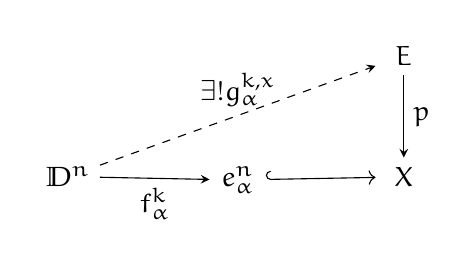
\begin{tikzpicture}
  \matrix (m) [matrix of math nodes,row sep=3em,column sep=4em,minimum width=2em]
  {
     &  & E \\
     \D^n & e_\alpha^n & X \\};
  \path[-stealth]
    (m-1-3) edge node [right] {$p$} (m-2-3)
    (m-2-1) edge node [below] {$f_\alpha^k$} (m-2-2)
    (m-2-2) edge [right hook->] node [below] {} (m-2-3)
    (m-2-1) edge [dashed] node [above] {$\exists!g_\alpha^{k,x}$}  (m-1-3);
\end{tikzpicture}
\end{center}
tal que $g_\alpha^{k,x}(0) = x$. Adem\'as, todo levantado de una funci\'on caracter\'istica es de \'esta forma, pues queda determinada un\'ivocamente por su imagen en cualquiera de sus puntos, en particular, en $0$. Ahora, afirmamos que $\mathcal{C} = \{c_\alpha^{k,x} := g_\alpha^{k,x}(\D^n) : k \in \natzero{n},\alpha \in J_k, x \in E_\alpha^k\}$ es una estructura celular:
\begin{itemize}
\item[\paint{grey-light-blue}{(i)}] $\bigcup_{c_\alpha^{k,y} \in \mathcal{C}}c_\alpha^{k,y} = E$ pues si $q \in E$, luego $p(q)  \in X$ pertenece a alguna celda $e_\alpha^k$. As\'i, es $p(q) = f_\alpha^k(z)$ para cierto $z \in \D^k$. Luego existe una \'unica funci\'on $g_\alpha^{k,y}$ tal que $g_\alpha^{k,y}(z) = q$. En consecuencia, es $q \in c_\alpha^{k,y}$.
\item[\paint{grey-light-blue}{(ii)}] Supongamos $\tint{{c_\alpha^{k,x}}} \cap \tint{{c_\beta^{l,y}}} \neq \emptyset$ y veamos que $\alpha = \beta, x = y, k = l$. Siempre es
\begin{align}
p(\tint{{c_\alpha^{k,x}}} \cap \tint{{c_\beta^{l,y}}}) \subset p(c_\alpha^{k,x} \cap c_\beta^{l,y}) \subset p(c_\alpha^{k,x}) \cap p(c_\beta^{l,y}) = e_\alpha^k \cap e_\beta^l. 
\end{align}
Veamos ahora que $p(\tint{{c_\alpha^{k,x}}} \cap \tint{{c_\beta^{l,y}}}) \subset \tint{{ e_\alpha^k}} \cap \tint{{e_\beta^l}}$. Como ya sabemos que vale $\paint{grey-light-blue}{(1)}$ y  $e_\alpha^k \cap e_\beta^l \subset \tint{{c_\beta^{l,y}}} \cap \tint{{ e_\alpha^k}} \cup \dot{e_\alpha^k} \cup \dot{e_\beta^l}$, es suficiente probar que
\begin{align}
p(\tint{{c_\alpha^{k,x}}} \cap \tint{{c_\beta^{l,y}}}) \subset \dot{e_\alpha^k}^c, \ \dot{e_\beta^l}^c.
\end{align}
Ambos casos son similares, lo hacemos para $e_\alpha^k$. Por el absurdo, si $p(q) \in \dot{e_\alpha^k}$, luego existe $e_\gamma^m$ tal que $p(q) \in e_\gamma^m$ y $m < k$. Existe entonces $g_\gamma^{m,w}$ tal que $g_\gamma^{m,w}(z) = q$ para cierto $z \in \D^m$ y as\'i $q \in c_\gamma^{m,w}$ con $m < k$, lo que es absurdo pues $q \in \tint{{c_\alpha^{k,x}}}$. En conclusi\'on, hemos probado $\paint{grey-light-blue}{(2)}$ y entonces siempre es $p(\tint{{c_\alpha^{k,x}}} \cap \tint{{c_\beta^{l,y}}}) \subset \tint{{ e_\alpha^k}} \cap \tint{{e_\beta^l}}$. Esto en particular implica que como $\tint{{c_\alpha^{k,x}}} \cap \tint{{c_\beta^{l,y}}} \neq \emptyset$, la intersecci\'on $\tint{{ e_\alpha^k}} \cap \tint{{e_\beta^l}}$ es no vac\'ia y entonces $\alpha = \beta, k = l$. Para terminar, veamos que $x = y$. Sea $q \in \tint{{c_\alpha^{k,x}}} \cap \tint{{c_\beta^{l,y}}} = \tint{{c_\alpha^{k,x}}} \cap \tint{{c_\alpha^{k,y}}}$. Luego existen $z,z' \in \D^k$ tales que 
\begin{align}
g_\alpha^{k,x}(z) = q = g_\alpha^{k,y}(z').
\end{align}
Aplicando $p$, tenemos
\begin{align*}
f_\alpha^k(z) = p(q) = f_\alpha^k(z'), 
\end{align*}
y como acabamos de probar que $p(q) \in \tint{{ e_\alpha^k}} = f_\alpha^k(\tint{(\D^k)})$, luego $z,z' \in \tint{(\D^k)}$. Restringida all\'i sabemos que $f_\alpha^k$ es biyectiva (de hecho, es un homeomorfismo con su imagen) as\'i que $z = z'$. Volviendo a $\paint{grey-light-blue}{(3)}$, tenemos dos levantados $g_\alpha^{k,x}, g_\alpha^{k,y}$ de $f_\alpha^k$ que coinciden en un punto y por lo tanto deben ser iguales. Finalmente, $x = g_\alpha^{k,x}(0) = g_\alpha^{k,y}(0) = y$.

\begin{center}
$\paint{grey-light-blue}{
\rule{400pt}{0.5pt}
}$
\end{center}

\item[]Antes de seguir observemos que tomando celdas iguales, en $\paint{grey-light-blue}{(ii)}$ probamos en particuar que $p(c_\alpha^{k,x}) \subset e_\alpha^{k,x}$ y $p(\tint{{c_\alpha^{k,x}}}) \subset \tint{{e_\alpha^{k,x}}}$ para cuaqluier celda.

\begin{center}
$\paint{grey-light-blue}{
\rule{400pt}{0.5pt}
}$
\end{center}

\item[\paint{grey-light-blue}{(iii)}] Afirmamos por \'ultimo que las correstricciones $g_\alpha^{k,y} : \D^k \to c_\alpha^{k,y}$ son funciones caracter\'isticas: debemos ver que $g_\alpha^{k,y}(\Ss^{k-1}) = \dot{c_\alpha^{k,x}}$, $g_\alpha^{k,y}(\tint{{\D^k}}) = \tint{{c_\alpha^{k,x}}}$ y que la restricci\'on $g_\alpha^{y,k} : \tint{{\D^k}} \to \tint{{c_\alpha^{y,k}}}$ es homeomorfismo.
\begin{itemize}
\item[$\blacktriangleright$] Si $x \in \Ss^{k-1}$ entonces $f_\alpha^k(x) \in \dot{e_\alpha^k}$ y por lo tanto $f_\alpha^k(x) \in e_\beta^m$ para cierta celda con $m < k$. Luego como $g_\alpha^{k,y}(x) \in E_{f_\alpha^k(x)}$, existe un levantado $g_\beta^{m,z}$ de $f_\beta^m$ tal que $g_\beta^{m,z}(x') = g_\alpha^{k,y}(x)$ para cierto $x' \in \D^{m}$. Por lo tanto $g_\alpha^{k,y}(x) \in c_\alpha^{k,x} \cap c_\beta^{m,z}$ y as\'i $g_\alpha^{k,y}(\Ss^{k-1}) \subset \dot{c_\alpha^{k,y}}$. Rec\'iprocamente, si $q = g_\alpha^{k,y}(x) \in c_\alpha^{k,y} \cap c_\beta^{m,w}$ para cierta celda con $m < k$ entonces $f_\alpha^k(x) = p(q) \in p(c_\alpha^{k,y}) \cap p(c_\beta^{m,w}) \subset \dot{e_\alpha^k}$. Por lo tanto, necesariamente es $x \in \Ss^{k-1}$ y entonces $\dot{c_\alpha^{y,k}} \subset g_\alpha^{k,y}(\Ss^{k-1})$.
\item[$\blacktriangleright$] Sea $x \in \tint{{\D^k}}$. Si su imagen por $g_\alpha^{k,y}$ no fuera parte del interior de $c_\alpha^{k,y}$, debe estar en el borde. Por lo tanto, por lo anterior existe $x' \in \Ss^{k-1}$ tal que $g_\alpha^{y,k}(x') = g_\alpha^{y,k}(x)$. Componiendo con $p$, luego es $f_\alpha^{k}(x') = f_\alpha^{k}(x)$ lo que es absurdo, pues este elemento ser\'ia imagen del borde e interior de $e_\alpha^k$ al mismo tiempo. Rec\'iprocamente, si $g_\alpha^{y,k}(x) \in \tint{{c_\alpha^{y,k}}}$ entonces $f_\alpha^k(x) = pg_\alpha^{k,y}(x) \in \tint{{e_\alpha^k}}$ y por lo tanto $x \in \tint{{\D^k}}$.
\item[$\blacktriangleright$] Sabemos que $g_\alpha^{y,k} : \tint{{\D^k}} \to \tint{{c_\alpha^{y,k}}}$ es continua y sobreyectiva. Como $f_\alpha^k$ es inyectiva en el interior del disco, tambi\'en tenemos la inyectividad: si $g_\alpha^{y,k}(x) = g_\alpha^{y,k}(x')$ para ciertos $x,x' \in \tint{{\D^k}}$ componiendo con $p$ es $f_\alpha^k(x) = f_\alpha^k(x')$ y entonces $x = x'$. Resta ver que $g_\alpha^{y,k}$ es abierta. Sea $U \subset \tint{{\D^k}}$ abierto, y veamos que $g_\alpha^k(U)$ es abierto. Por hip\'otesis, $f_\alpha^k(U)$ es abierto en $\tint{{e_\alpha^k}}$, es decir tenemos que $f_\alpha^k(U) = V \cap \tint{{e_\alpha^k}}$ con $V$ abierto en $X$. Luego $p^{-1}(V)$ es abierto y afirmamos entonces que $g_\alpha^{k,y}(U) = p^{-1}(V) \cap \tint{{c_\alpha^{k,y}}}$. Ya sabemos que $g_\alpha^{k,y}(U) \subset \tint{{c_\alpha^{k,y}}}$, y adem\'as $pg_\alpha^{k,y}(U) = f_\alpha^k(U) \subset V$ as\'i que $g_\alpha^{k,y}(U) \subset p^{-1}(V)$. Veamos la otra contenci\'on: sea $y \in p^{-1}(V) \cap \tint{{c_\alpha^{k,y}}}$. Como $g_\alpha^{k,y}$ es una biyecci\'on entre el interior del disco y de la celda, luego $y \in p^{-1}(V) \cap \tint{{c_\alpha^{k,y}}}$ si y s\'olo si $y = g_\alpha^{k,y}(x)$ con $p(y) = f_\alpha^k(x) \in V$ y $x \in \tint{{\D^k}}$. Una vez m\'as, como $f_\alpha^k$ es una biyecci\'on entre el interior del disco y el interior de $e_\alpha^k$, esto equivale a decir que $f_\alpha^k(x) \in V \cap \tint{{e_\alpha^k}} = f_\alpha^k(U)$. En particular $x$ debe ser un elemento del interior del disco, y como $f_\alpha^k$ es biyectiva en $U$, luego es $x \in U$ e $y = g_\alpha^{k,y}(x) \in g_\alpha^{k,y}(U)$. 
\end{itemize}
\end{itemize}
Esto termina la demostraci\'on de que $E$ admite una estructura celular. Veamos ahora que es CW-complejo, es decir, que cumple las propiedades (C) y (W).
\begin{itemize}
\item[$\blacktriangleright$] \underline{$E$ verifica $(C)$:} si $c_\beta^{l,y} < c_\alpha^{k,x}$ entonces $e_\alpha^l < e_\beta^k$ pues
\begin{align*}
p({c_\alpha^{k,x}} \cap \tint{{c_\beta^{l,y}}}) \subset p(c_\alpha^{k,x}) \cap p(\tint{{c_\beta^{l,y}}}) \subset e_\alpha^k \cap \tint{{e_\beta^l}},
\end{align*}
y m\'as a\'un de aqu\'i se ve que si $c_\beta^{l,y}$ es cara de $c_\alpha^{k,x}$ entonces $e_\alpha^l$ es cara de  $e_\beta^k$. Entonces, si $c_\beta^{l,y}$ tuviese infinitas caras, tendr\'iamos al menos numerables celdas $\{c_{\alpha_n}^{k_n,y_n}\}_{n \geq 1}$ que son caras de $c_\beta^{l,y}$. Luego las celdas $\{e_{\alpha_n}^{k_n}\}_{n \geq 1}$ ser\'ian caras de $e_\beta^l$ y como $X$ es CW-complejo, deben ser finitas: as\'i, las suceciones $(\alpha_n)_n,(k_n)_n$ toman finitos valores $\gamma_1, \dots, \gamma_s$ y $m_1, \dots, m_r$. Luego, debe existir un par $(\gamma_i,k_j)$ tal que hay infinitas celdas de la forma $c_{\gamma_i}^{k_j,x}$ que son caras de $c_\beta^{l,y}$. \textbf{[Me falt\'o probar que esto \'ultimo es absurdo. Una idea que tuve, pero que no pude conretar, fue intentar ver que algunos de estos puntos formaban un subespacio discreto y usar la compacidad de $c_\alpha^{l,y}$]}
\item[$\blacktriangleright$] \underline{$E$ verifica $(W)$}: cada celda $c_\alpha^{k,y}$ es compacta en $E$ Hausdorff as\'i que es cerrada, y en particular si $F \subset E$ es cerrado entonces $F \cap c_\alpha^{k,y}$ es cerrado para cada $c_\alpha^{k,y}$. Equivalentemente un abierto en $E$ es abierto en cada celda. Debemos ver la rec\'iproca: supongamos que $U \subset E$ es tal que $U \cap c_\alpha^{k,y}$ es abierto para toda celda $c_\alpha^{k,y}$ y veamos que $U$ es abierto. \textbf{[No pude completar la prueba: una idea que no pude llevar a cabo era considerar las preimagenes de abiertos parejamente cubiertos. Como cubren $E$, alcanza ver que $U$ es abierto al intersecarlo con cada una de \'estas, y de ah\'i se podr\'ia intentar "pasar el problema a uno en $X$" y usar que \'este tiene la topolog\'ia final con respecto a sus celdas]}
\end{itemize}
Esto termina de probar que $E$ es un CW-complejo, y es de dimensi\'on $n$ por construimos su estructura celular. Finalmente, veamos que un CW-complejo arcoconexo siempre admite un revestimiento universal. Para esto, basta probar que los CW-complejos son localmente arcoconexos y semi-localmente simplemente conexos. Como cada celda es localmente arcoconexa y "ser localmente arcoconexo" es una propiedad cerrada por cocientes y uniones disjuntas, en particular el $0$-esqueleto es localmente arconocexo. M\'as a\'un, inductivamente todo $k$-esqueleto es localmente arcoconexo pues es un cociente de una uni\'on disjunta de espacios localmente arcoconexos. Por \'ultimo, eso dice que $\sqcup_{k \geq 0}X^{(k)}$ es arcoconexo, y como $q : x \in X^{(s)} \subset \sqcup_{k \geq 0}X^{(k)} \mapsto x \in X^{(s)} \subset X$ es cociente pues $X$ tiene la topolog\'ia final respecto de las inclusiones de cada esqueleto, luego $X$ es un cociente de un espacio localmente arcoconexo: en particular, $X$ es localmente arcoconexo. \textbf{[Me falt\'o probar que los CW-complejos son semi-localmente simplemente conexos]}
\end{proof}

\end{document}
